% Drawing 154/01-9 -- folder 154, batch 01, archive page 14 (PDF page 15).
% Transcription: figure : deux faisceaux de pseudo-droites orange, reliés par une droite orange ; de part et d'autre, des bandes jaunes et vertes, en trait plein et en pointillé, suivent la droite et s'écartent aux sommets, deux petites flèches doubles marquant l'écart
% Kind: two pencils on a line, with parallel bands. Method 2 (schematic redraw from the facsimile). Status: ok.
% Notes: Two pencils of orange pseudolines (two and three lines) on a long orange line, with a marked point between them; yellow and green bands, solid and dotted, follow the line on both sides, crossing it at the middle point and spreading at the vertices; two small double arrows mark the gap. The band strokes are drawn as single curves (his pairs of strokes merged where they run together).
% Coordinates: 1 unit = 1 mm = 1/100 of the crop width (bbox in page fractions: [0.121, 0.361, 0.474, 0.451]).
% Redrawn by Claude (claude-opus-5-5), issue #73, 2026-11-07; not checked by a human; not compiled (no TeX in the session).
% Rights: reproduces part of the work -- behind RENDER_TRANSCRIPTS, never published by itself.
\documentclass[tikz,border=3pt]{standalone}
\usepackage{amsmath,amssymb}
\usetikzlibrary{patterns,arrows.meta}
\tikzset{Or/.style={orange!90!black}, Ye/.style={yellow!80!orange}, Lg/.style={green!60!black!70}, Dg/.style={green!45!black}, Br/.style={brown!80!black}, Rd/.style={red!85!black}, Bl/.style={blue!70!black}, Gy/.style={black!40}, pencil/.style={black!45}, struck/.style={black!35}, mark/.style={circle,draw,inner sep=1.3pt}, pt/.style={circle,fill,inner sep=0.9pt}, opt/.style={circle,draw,fill=white,inner sep=1.1pt}}
\begin{document}
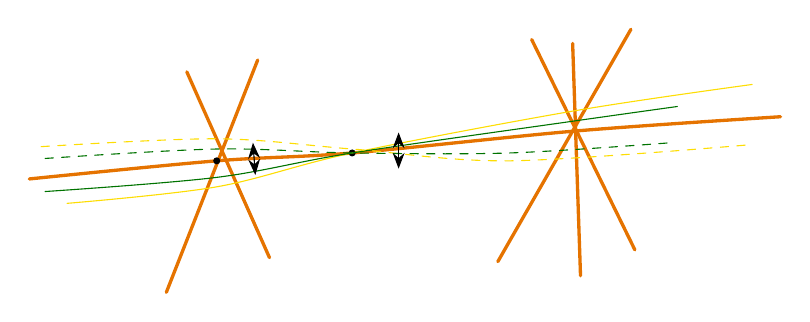
\begin{tikzpicture}[x=1mm,y=1mm,line cap=round,line join=round,font=\scriptsize]
\draw[Or,very thick] plot[smooth, tension=0.55] coordinates {(3.1,-20.5) (26.9,-18.2) (44.1,-17.2) (72.6,-14.4) (98.5,-12.6)};
\draw[Or,very thick] (23.1,-6.9) -- (33.6,-30.5);
\draw[Or,very thick] (32.1,-5.4) -- (20.5,-34.9);
\draw[Or,very thick] (66.9,-2.8) -- (80,-29.5);
\draw[Or,very thick] (79.5,-1.5) -- (62.6,-31);
\draw[Or,very thick] (72.1,-3.3) -- (73.1,-32.8);
\node[pt] at (26.9,-18.2) {};
\node[pt] at (44.1,-17.2) {};
\draw[Ye] plot[smooth, tension=0.55] coordinates {(7.9,-23.6) (26.9,-21.5) (44.1,-17.2) (72.6,-11.8) (94.9,-8.5)};
\draw[Dg] plot[smooth, tension=0.55] coordinates {(5.1,-22.1) (26.9,-20.3) (44.1,-17.2) (72.6,-13.1) (85.4,-11.3)};
\draw[Ye,dashed] plot[smooth, tension=0.55] coordinates {(4.6,-16.4) (26.9,-15.4) (44.1,-16.7) (64.1,-18.2) (94.1,-16.2)};
\draw[Dg,dashed] plot[smooth, tension=0.55] coordinates {(5.1,-17.9) (26.9,-16.7) (44.1,-17.2) (64.1,-17.2) (84.6,-15.9)};
\draw[{Stealth[length=2mm]}-{Stealth[length=2mm]}] (31.5,-15.9) -- (31.8,-20);
\draw[{Stealth[length=2mm]}-{Stealth[length=2mm]}] (50,-14.6) -- (50,-19.2);
\end{tikzpicture}
\end{document}
